\chapter{Ping}

O pacote ping é um programa que envia pacotes do cliente para o servidor e para
cada pacote enviado é recebido um pacote como resposta e retorna o delay desse
processo, esse delay é nomeado como RTT, Round Trip Time, se esse delay
ultrapassa um certo limite de tempo o programa ping responde que o pacote foi
perdido e não houve conexão.

A execução do programa ping utilizando o argumento www.google.com.br pode ser
visualizada na figura~\ref{fig:ping_result}.

\begin{figure}[h]
  \centering
  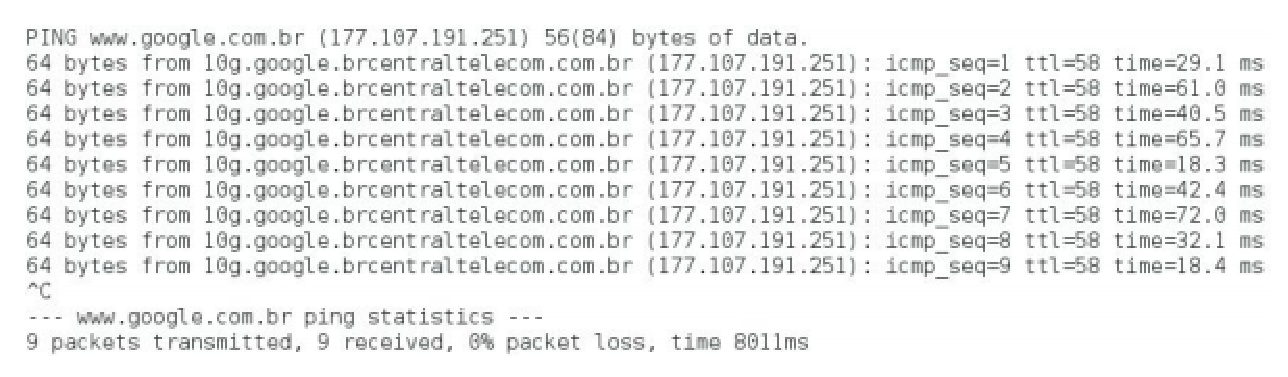
\includegraphics[width=0.9\textwidth]{figuras/ping_result.eps}
  \caption{Saída do comando ping www.google.com.br}
  \label{fig:ping_result}
\end{figure}

A ferramenta utilizada foi o wireshark que permite selecionar um host através
do seu endereço IP e monitorar todos os pacotes que possuem o IP do host como
endereço de origem ou endereço de destino, através desse monitoramento é
possível identificar os protocolos utilizados no envio dos pacotes e suas
mensagens. A figura~\ref{fig:wireshark_result} mostra a execução do programa
wireshark.

\begin{figure}[h]
  \centering
  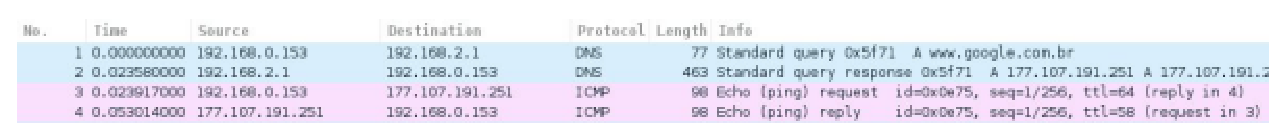
\includegraphics[width=0.9\textwidth]{figuras/wireshark.eps}
  \caption{Resultado da execução do programa wireshark}
  \label{fig:wireshark_result}
\end{figure}

O seguinte processo descreve a execução do programa ping mostrando os
protocolos utilizados na camada de transporte e de rede, e também
ilustrando de forma simples os dados dos pacotes enviados pela rede.
Nesse precosso o cliente é o computador com IP 192.168.0.153, e o
servidor é o site www.google.com.br.

O cliente envia um pacote UDP para o DNS, utilizando o protocolo
IP, solicitando o IP do endereço “www.google.com.br”, o pacote é ilustrado
na figura~\ref{fig:pkg_client_to_dns}.

    \begin{figure}[h]
      \centering
      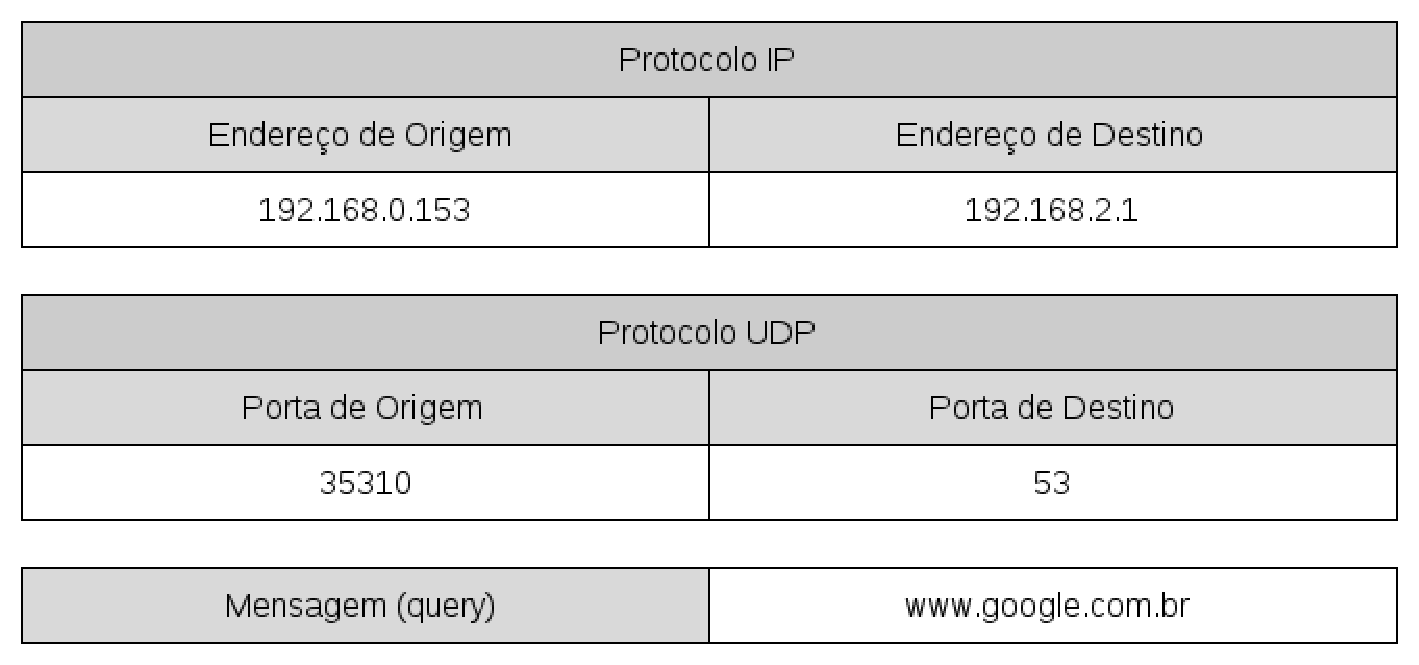
\includegraphics[width=0.9\textwidth]{figuras/pkg_client_to_dns.eps}
      \caption{Pacote enviado do cliente para o DNS}
      \label{fig:pkg_client_to_dns}
    \end{figure}

O DNS também responde para o cliente com um pacote UDP, utilizando
o protocolo IP, enviando uma mensagem com o endereço IP do nome
“www.google.com.br”, o pacote é ilustrado na figura~\ref{fig:pkg_dns_to_client}.

    \begin{figure}[h]
      \centering
      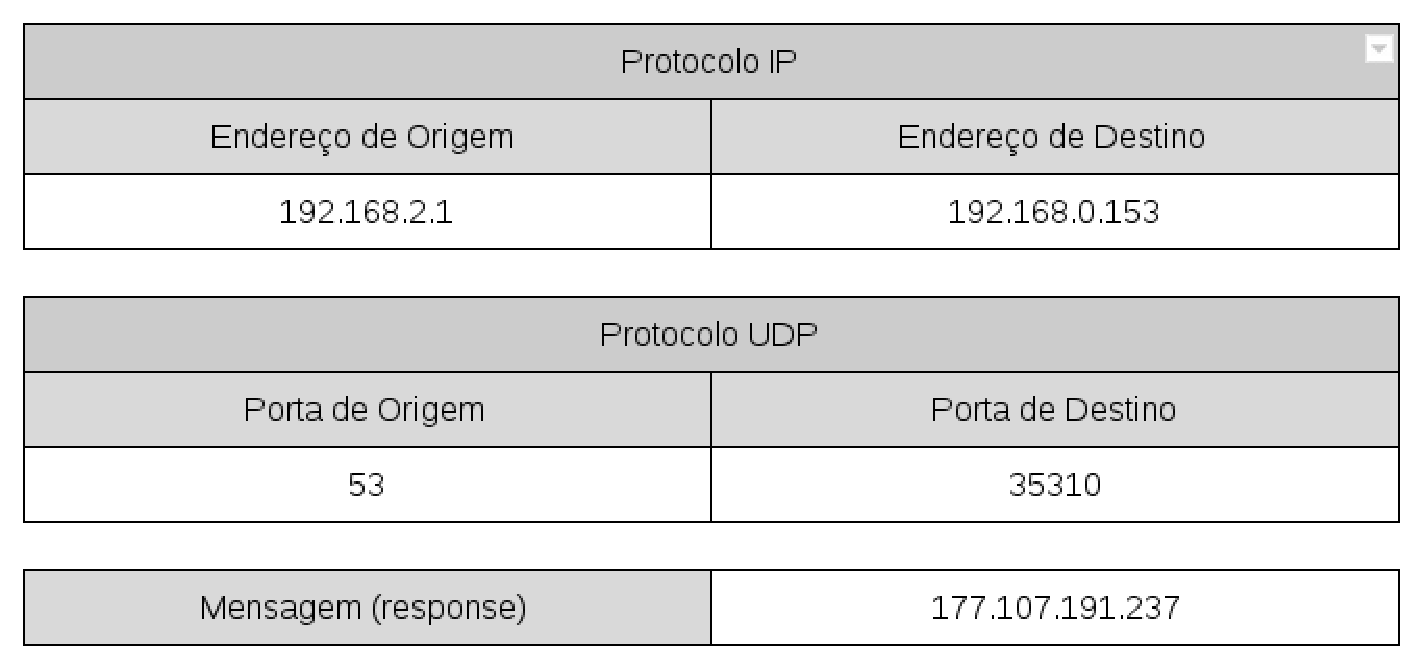
\includegraphics[width=0.9\textwidth]{figuras/pkg_dns_to_client.eps}
      \caption{Pacote enviado do DNS para o cliente}
      \label{fig:pkg_dns_to_client}
    \end{figure}

O cliente envia uma mensagem para o servidor utilizando o protocolo ICMP,
através do protocolo IP, ilustrado na figura~\ref{fig:pkg_client_to_server}.

    \begin{figure}[h]
      \centering
      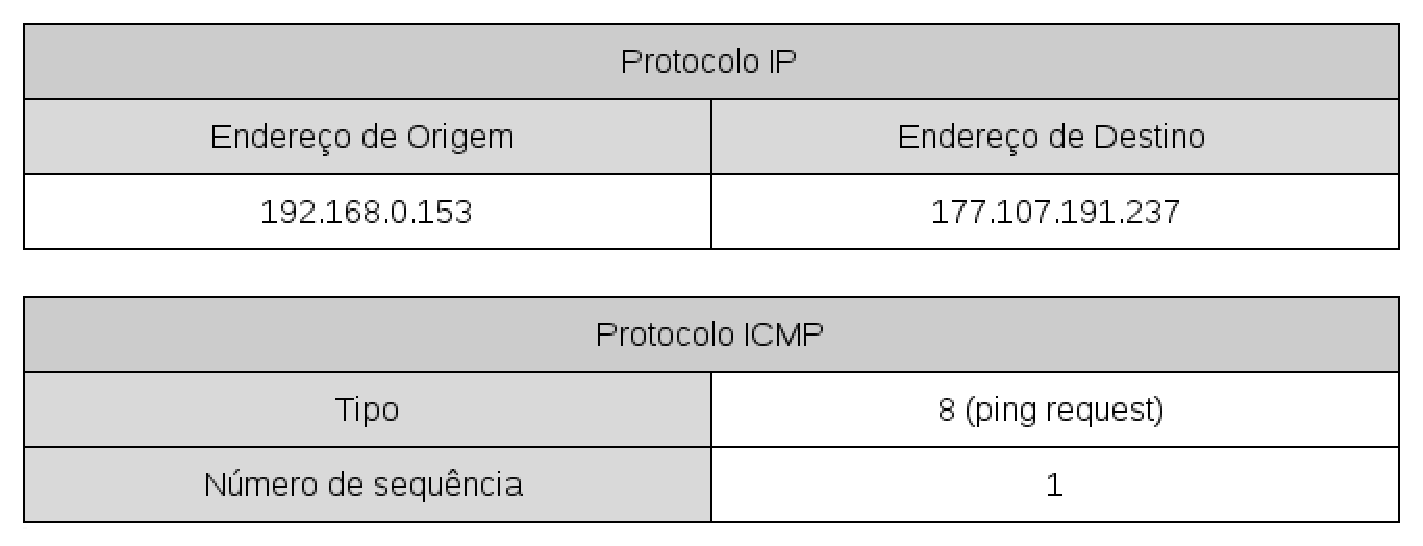
\includegraphics[width=0.9\textwidth]{figuras/pkg_client_to_server.eps}
      \caption{Pacote enviado do cliente para o DNS}
      \label{fig:pkg_client_to_server}
    \end{figure}

O servidor responde o cliente com um pacote, também utilizando o ICMP
através do protocolo IP, ilustrado na figura~\ref{fig:pkg_server_to_client}.

    \begin{figure}[h]
      \centering
      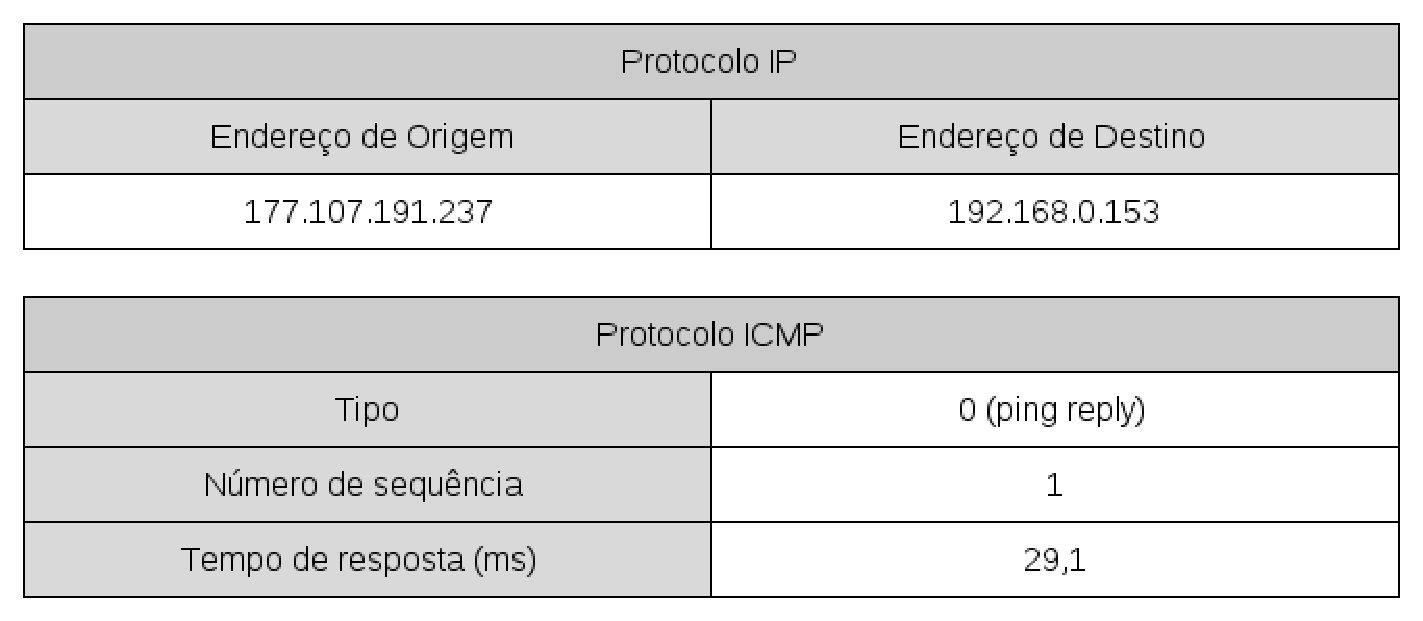
\includegraphics[width=0.9\textwidth]{figuras/pkg_server_to_client.eps}
      \caption{Pacote enviado do DNS para o cliente}
      \label{fig:pkg_server_to_client}
    \end{figure}

Nesse experimento foram enviados 9 pacotes e 9 pacotes foram recebidos
pelo ping, logo não ocorreu perda de pacote, as figuras~\ref{fig:pkg_icmp_seq_2}
\ref{fig:pkg_icmp_seq_3}~\ref{fig:pkg_icmp_seq_4} mostram um resumo do
tráfego de pacotes através das transmissões desses 18 pacotes, onde cada
figura apresenta um par que contém o pacote enviado e o pacote recebido.

    \begin{figure}[h]
      \centering
      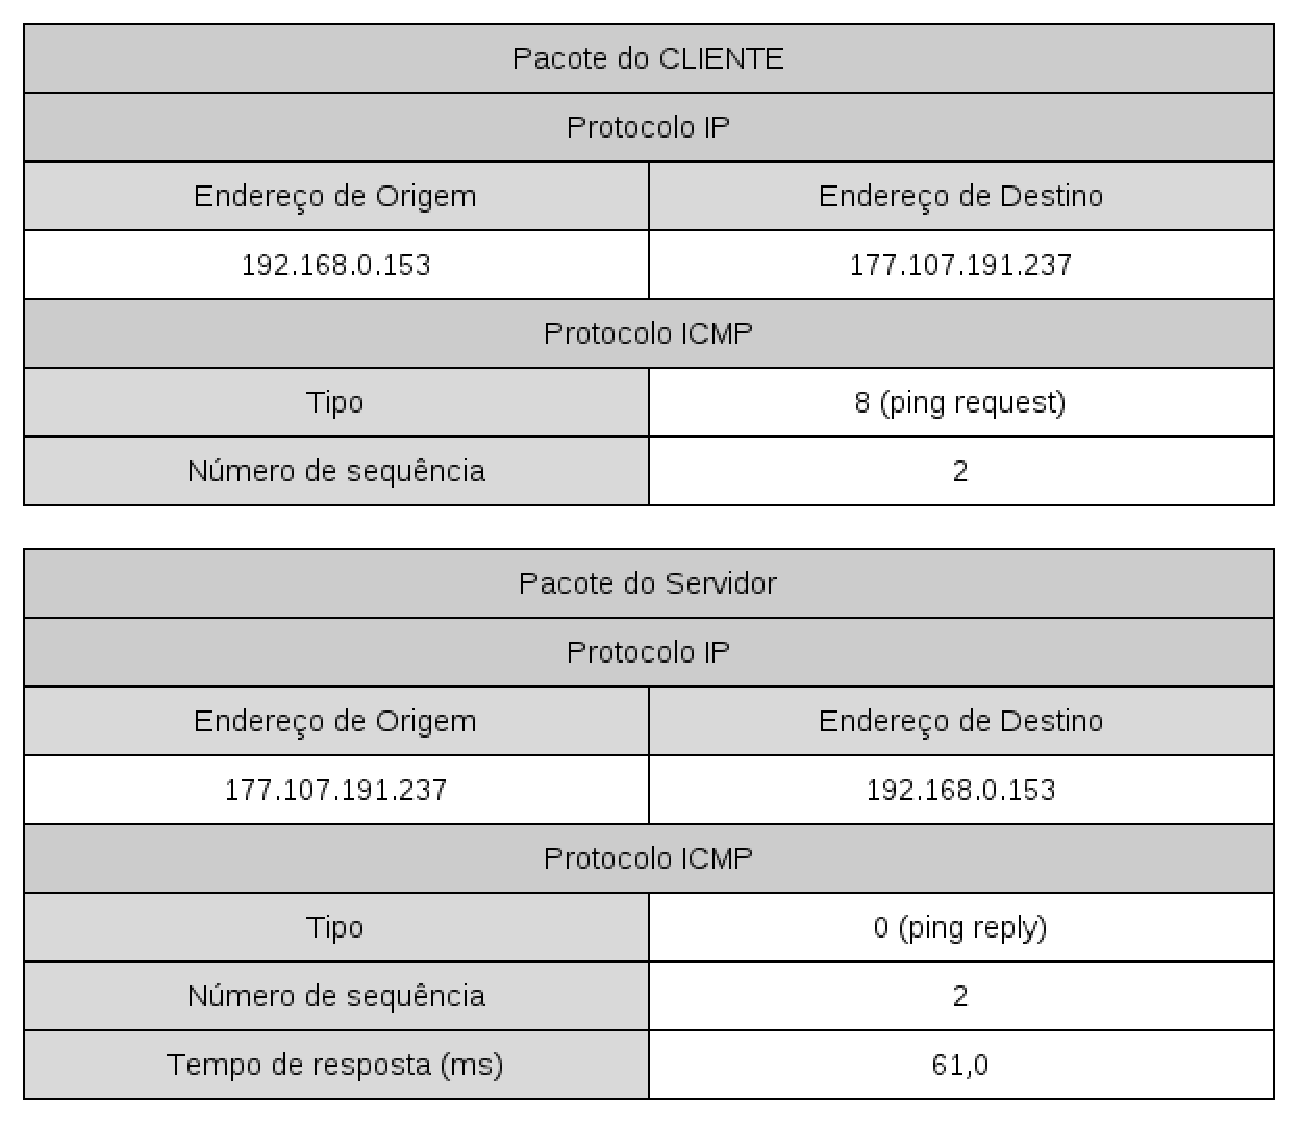
\includegraphics[width=0.9\textwidth]{figuras/pkg_icmp_seq_2.eps}
      \caption{Pacotes ICMP com número de sequência 2}
      \label{fig:pkg_icmp_seq_2}
    \end{figure}

    \begin{figure}[h]
      \centering
      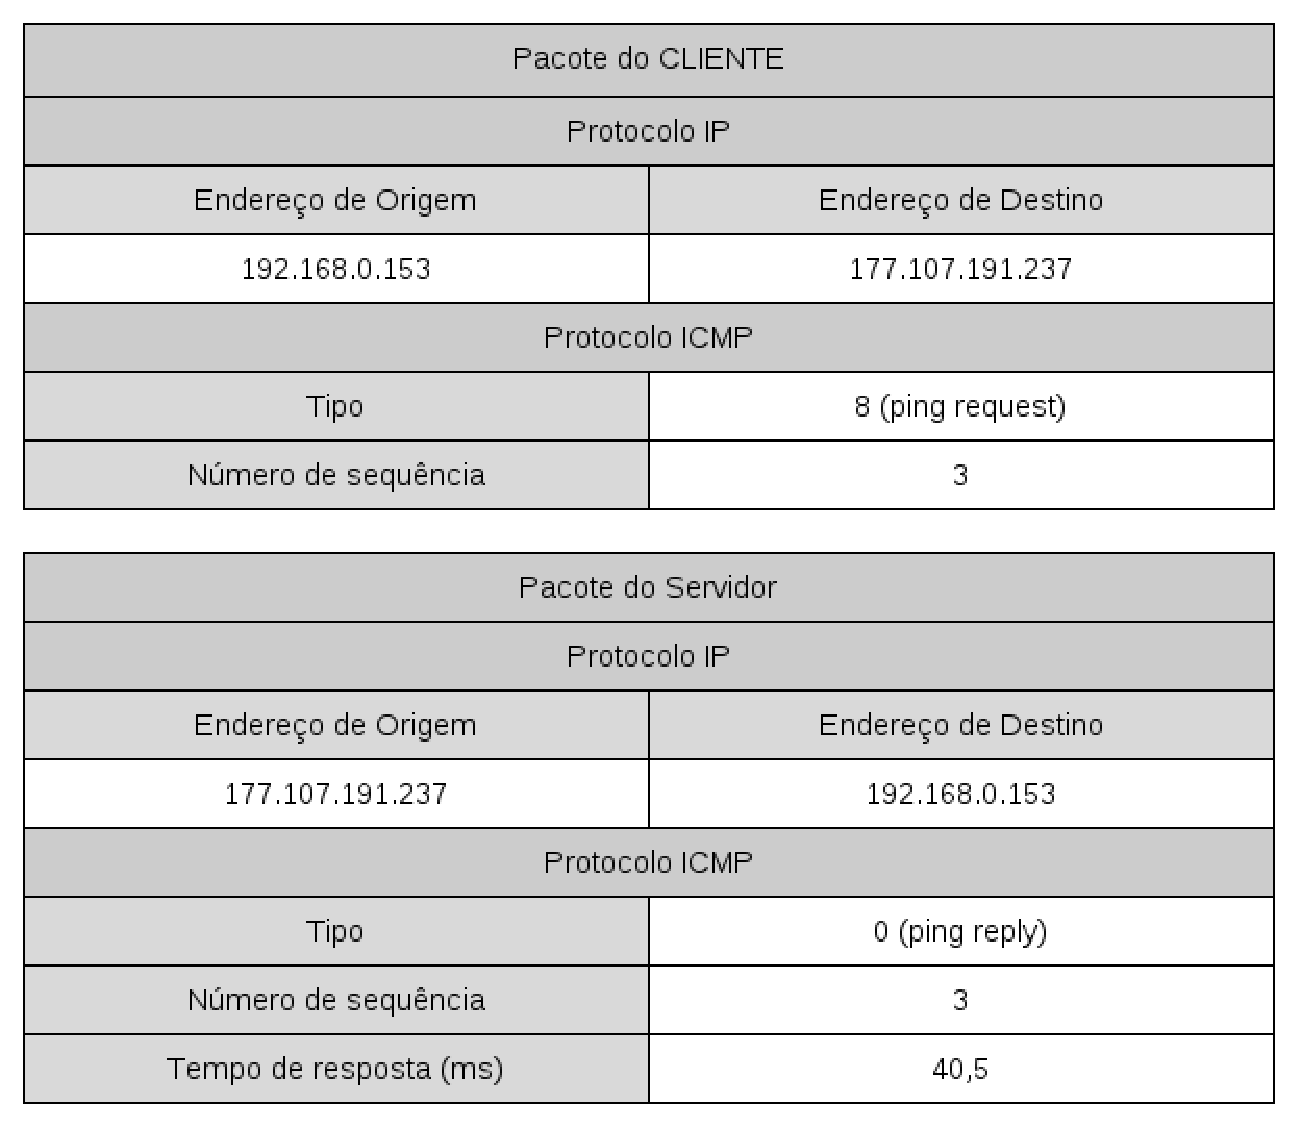
\includegraphics[width=0.9\textwidth]{figuras/pkg_icmp_seq_3.eps}
      \caption{Pacotes ICMP com número de sequência 3}
      \label{fig:pkg_icmp_seq_3}
    \end{figure}

    \begin{figure}[h]
      \centering
      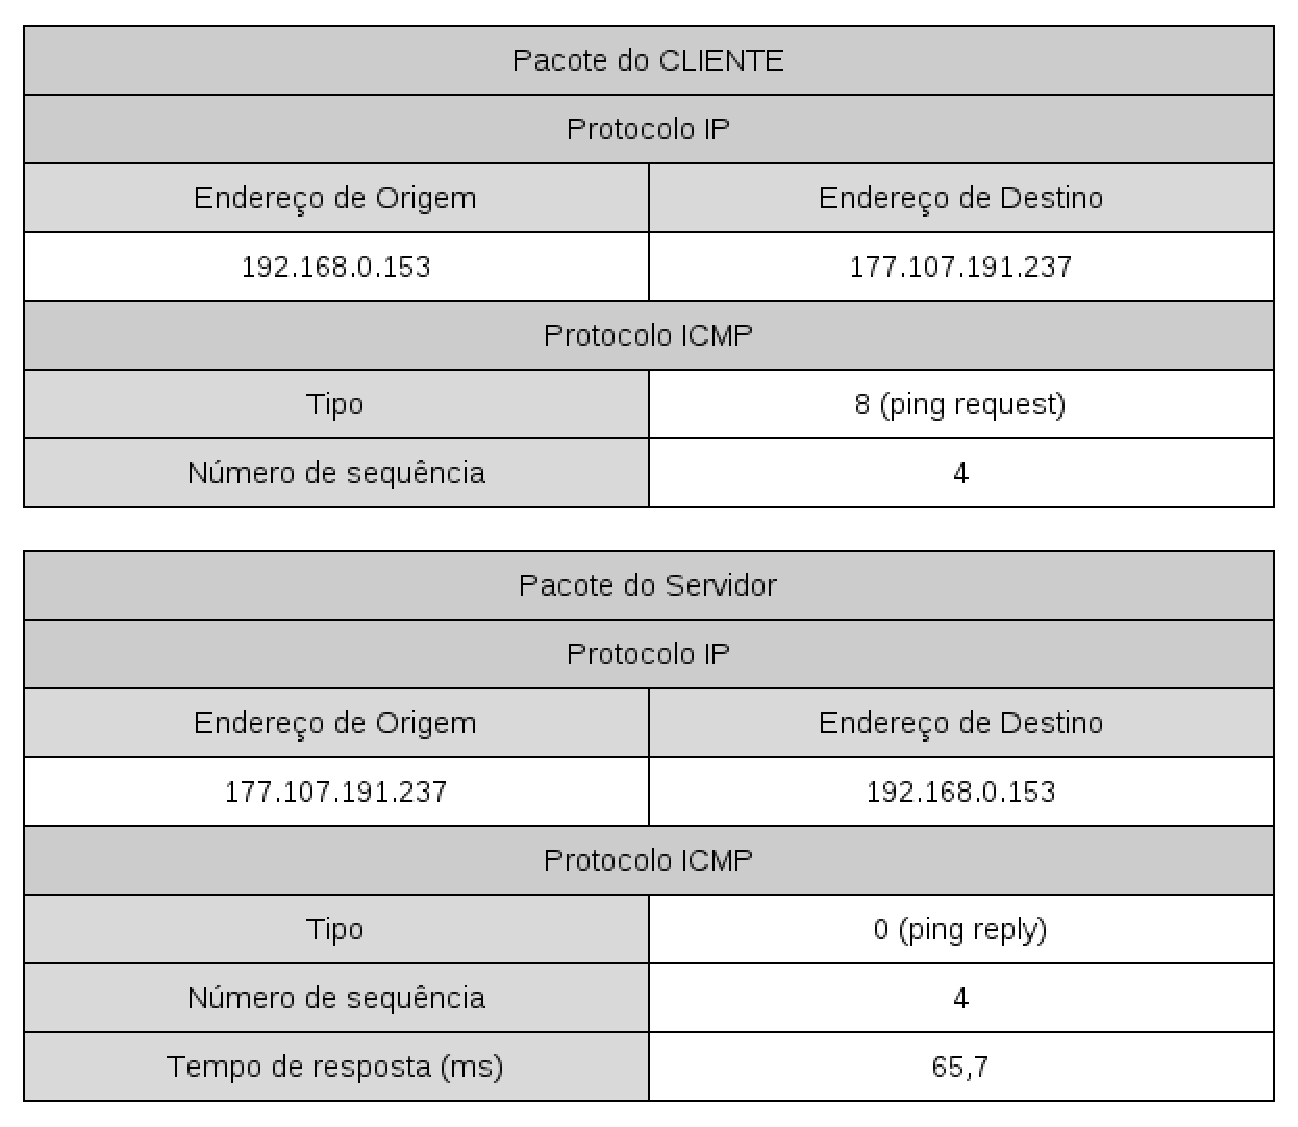
\includegraphics[width=0.9\textwidth]{figuras/pkg_icmp_seq_4.eps}
      \caption{Pacotes ICMP com número de sequência 4}
      \label{fig:pkg_icmp_seq_4}
    \end{figure}
